%!TEX root = Main.tex
\documentclass[Main]{subfiles}

\begin{document}

\section{System Description} % (fold)
\label{sec:system_description}

	This section will cover the overall system description
	
	\subsection{Block Definition Diagram} % (fold)
	\label{sub:system_bdd}

		Describe the BDD and the overall structure
	
		\begin{figure}[H]
			\centering
			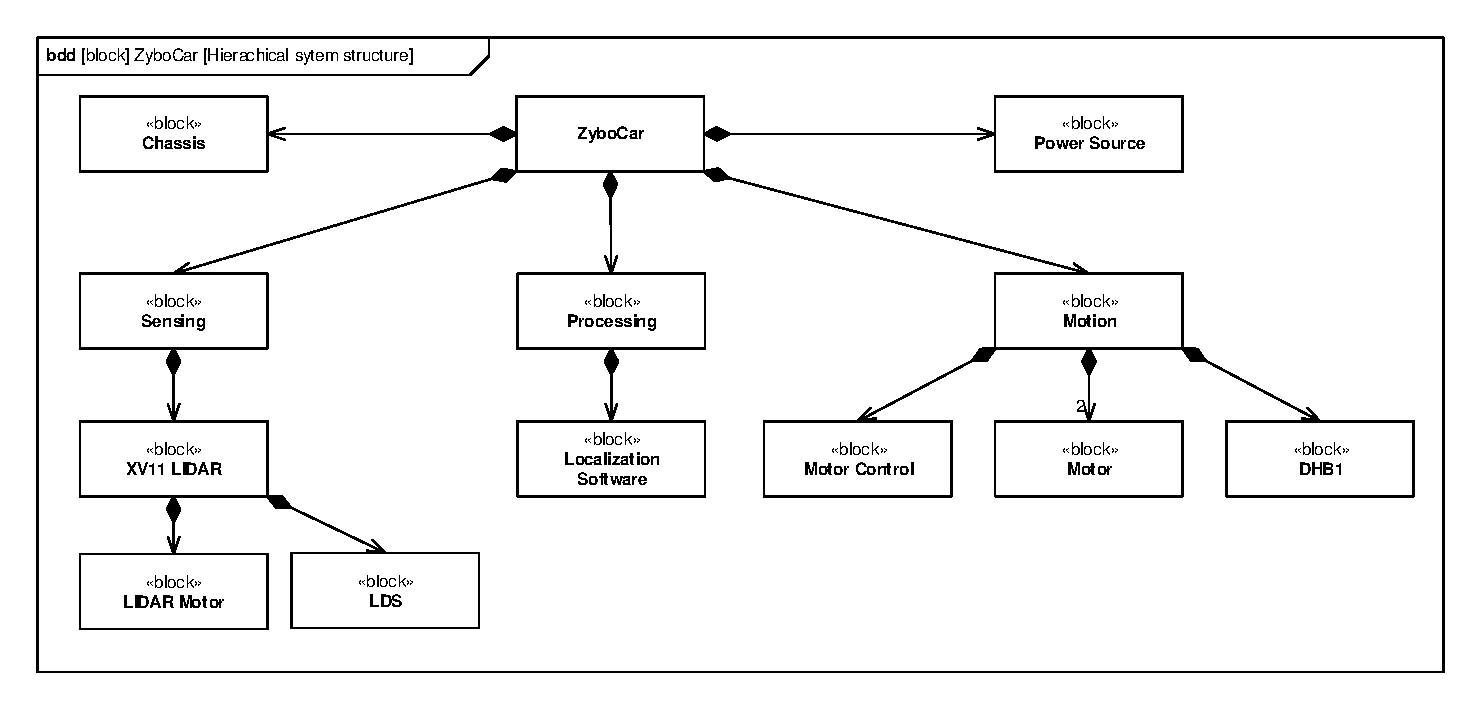
\includegraphics[width=\linewidth]{SystemBDD}
			\caption{System Block Diagram}
			\label{fig:systembdd}
		\end{figure}
		
	\subsection{Internal Block Diagram} % (fold)
	\label{sub:system_ibd}
	
		Describe the IBD and the flow of data
		\begin{figure}[H]
			\centering
			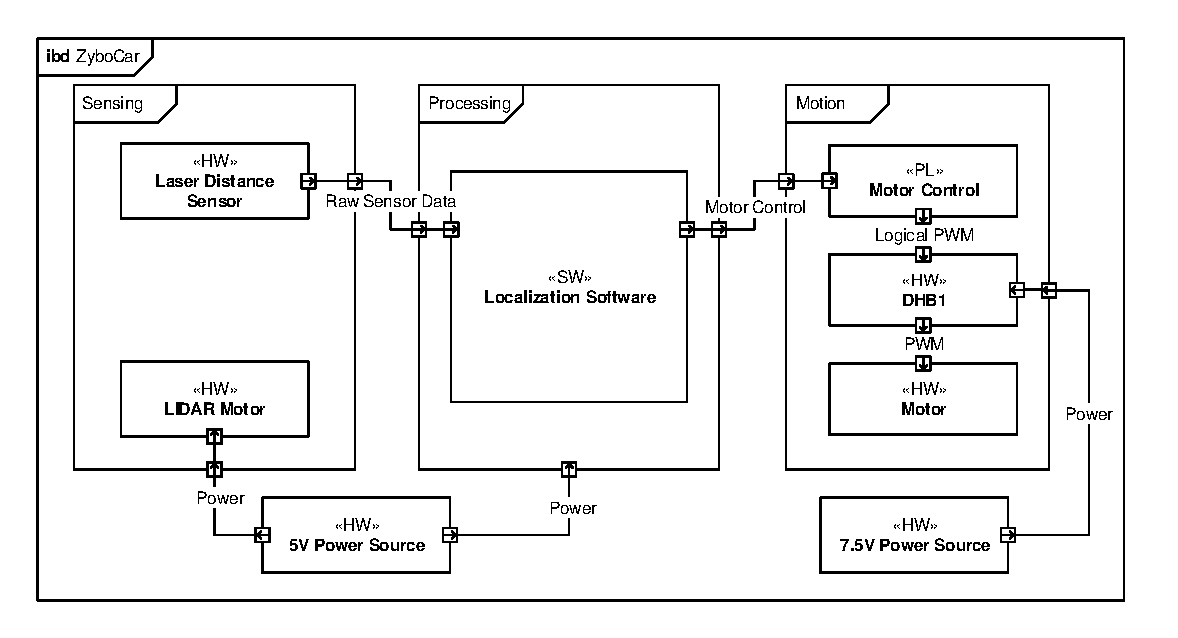
\includegraphics[width=\linewidth]{SystemIBD}
			\caption{System Internal Block Diagram}
			\label{fig:systemibd}
		\end{figure}

	\subsection{Activity Diagram} % (fold)
	\label{sub:system_act}
	
		Describe the ACT and the behaviour of the system
		\begin{figure}[H]
			\centering
			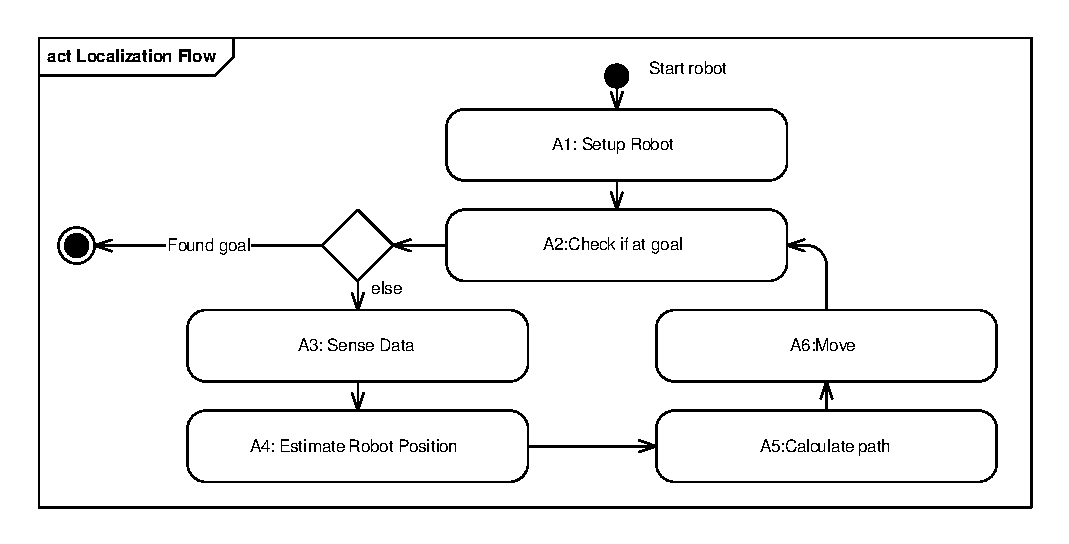
\includegraphics[width=\linewidth]{SystemACT}
			\caption{System Activity Diagram}
			\label{fig:systemact}
		\end{figure}

% section system_description (end)
\end{document}